\usepackage{xcolor}
\usepackage{afterpage}
\usepackage{hyperref}
\usepackage{caption}
\usepackage{pifont,mdframed}
\usepackage[bottom]{footmisc}

\makeatletter
\gdef\this@inputfilename{input.txt}
\gdef\this@outputfilename{output.txt}
\makeatother

\newcommand{\inputfile}{\texttt{input.txt}}
\newcommand{\outputfile}{\texttt{output.txt}}

\newenvironment{warning}
  {\par\begin{mdframed}[linewidth=2pt,linecolor=gray]%
    \begin{list}{}{\leftmargin=1cm
                   \labelwidth=\leftmargin}\item[\Large\ding{43}]}
  {\end{list}\end{mdframed}\par}

  A recent study confirmed the existence of gravitational waves. This extraordinary discovery has led more and more people to become interested in space. Sadly, space is still quite unreachable for common people. William is a bit depressed by this fact, but he's positive that he can exploit this media attention to advertise a new business. He decided to launch a startup for interstellar travel.

  It's important to note, though, that stars can be quite far. The \emph{Sun} is the star that's closest to us, but the others are pretty far. \emph{Proxima Centauri}, the ``second nearest star'', is $4.24$ light years away from the Sun: that means that it would take well over four years to reach this star! (assuming we know how to travel at the speed of light).

  \begin{figure}[h]
    \centering
    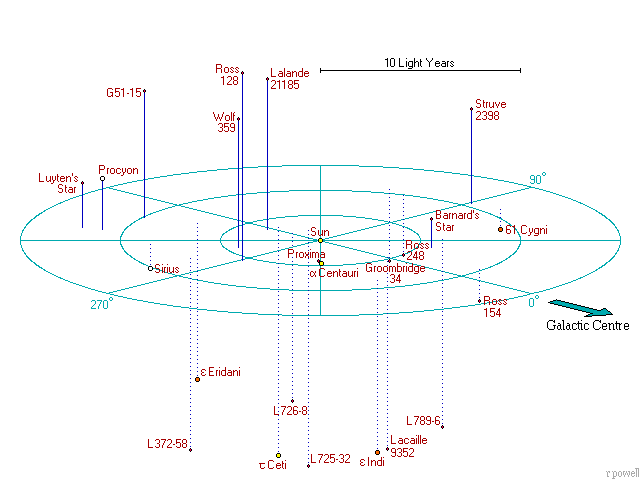
\includegraphics[width=0.8\textwidth]{12ly.png}
    \caption*{There are $33$ stars within $12.5$ light years from the Sun \\ \scriptsize (Richard Powell \href{http://creativecommons.org/licenses/by-sa/2.5}{CC BY-SA 2.5} via Wikimedia Commons)}
  \end{figure}

  William believes he can build a spaceship that is able to travel at the speed of light (he's found \href{https://www.youtube.com/watch?v=dQw4w9WgXcQ}{a YouTube tutorial} that seemed quite trustworthy), so he went on and bought a telescope to trace a 3D map of the Milky Way. Each star is specified in the 3D map through a $(x, y, z)$ point in space. The Sun is always in the map, and it's always specified by $(0, 0, 0)$.

  Write a program that, given the 3D sky map, is able to answer $Q$ queries: each query has an integer $D$, and must be answered with the number of stars that can be reached assuming that $D$ will be spent for travelling.

\Implementation
You shall submit exactly one file having extension \texttt{.c}, \texttt{.cpp} o \texttt{.pas}.

\begin{warning}
Among the attachments of this task you will find a template (\texttt{annoluce.c}, \texttt{annoluce.cpp}, \texttt{annoluce.pas}) with a sample incomplete implementation.
\end{warning}

If you use the template, you'll need to implement the following functions:
\begin{center}\begin{tabularx}{\textwidth}{|c|X|}
\hline
C/C++  & \begin{tabular}[x]{@{}@{}}\verb|void mappatura(int N, int X[], int Y[], int Z[]);|\\ \verb|int query(int D);|\end{tabular}\\
\hline
Pascal & \begin{tabular}[x]{@{}@{}}\verb|procedure mappatura(N: longint; var X, Y, Z: array of longint);|\\ \verb|function query(D: longint) : longint;|\end{tabular}\\
\hline
\end{tabularx}\end{center}
Where:
\begin{itemize}[nolistsep]
  \item The integer $N$ is the number of stars in the sky map.
  \item Arrays \texttt{X}, \texttt{Y} and \texttt{Z}, indexed from $0$ to $N-1$, contain the coordinates of the $N$ stars. That is: the $i$-th star is located at (\texttt{X[i]}, \texttt{Y[i]}, \texttt{Z[i]}).
  \item The \texttt{mappatura} function will only be called once, at the start of the program.
  \item Each call to \texttt{query(D)} must return the number of stars within $D$ light years from the Sun.
\end{itemize}

\InputFile
File \inputfile{} consists of $N+Q+2$ lines. The first line contains the single integer $N$. The next $N$ lines contain the coordinates $X_i, Y_i, Z_i$ of the $i$-th star, separated by spaces. The next line contains the single integer $Q$. The next $Q$ lines contain the values of $D$ for the relevant queries.

\OutputFile
File \outputfile{} consists of $Q$ lines containing an integer each: the answer for the relevant query.

% Assunzioni
\Constraints
\begin{itemize}[nolistsep, itemsep=2mm]
  \item $1 \le N, Q \le 100\,000$.
  \item $0 \le X_i, Y_i, Z_i < 2^{30}$ for each $i=0\ldots N-1$.
  \item The unit of measure for $x, y, z$ axes is the light year.
  \item $0 \le D < 2^{31}$ for each call to \texttt{query(D)}.
  \item The $D$ value is expressed in light years.
\end{itemize}

\Scoring
Your program will be tested against several test cases grouped in subtasks.
In order to obtain a subtask's score, your program needs to correctly solve all of its test cases.

\pagebreak

\begin{itemize}[nolistsep,itemsep=2mm]
  \item \textbf{\makebox[2cm][l]{Subtask 1} [10 points]}: Sample test cases.
  \item \textbf{\makebox[2cm][l]{Subtask 2} [20 points]}: $\mathtt{Y[i]} = \mathtt{Z[i]} = 0$ for each $i$. Instead of being in a tridimensional space, every star lie on the same line!
  \item \textbf{\makebox[2cm][l]{Subtask 3} [20 points]}: $\mathtt{Z[i]} = 0$ for each $i$. Instead of being in a tridimensional space, we're in bidimensional plane!
  \item \textbf{\makebox[2cm][l]{Subtask 4} [10 points]}: $N, Q, D \le 10$.
  \item \textbf{\makebox[2cm][l]{Subtask 5} [10 points]}: $N \le 100$; $D < 10\,000$.
  \item \textbf{\makebox[2cm][l]{Subtask 6} [10 points]}: $Q \le 100$; $D < 10\,000$.
  \item \textbf{\makebox[2cm][l]{Subtask 7} [20 points]}: No limits.
\end{itemize}

% Esempi


\Examples
\begin{example}
\exmpfile{annoluce.input0.txt}{annoluce.output0.txt}%
\exmpfile{annoluce.input1.txt}{annoluce.output1.txt}%
\end{example}


\Explanation
In the \textbf{first sample test case}, the $3$ stars are respectively: $0$ light years, $\sqrt{3}$ light years and $2\sqrt{3}$ light years away from the Sun. \\[2mm]
In the \textbf{second sample test case}, the $5$ stars are respectively: $\sqrt{14}$ light years, $\sqrt{77}$ light years, $0$ light years, $9\sqrt{3}$ light years and $\sqrt{51}$ light years away from the Sun.
